\documentclass{article}
\usepackage[utf8]{inputenc}

\usepackage{ifxetex}
\ifxetex
  \usepackage{fontspec}
\else
  \usepackage[T1]{fontenc}
  \usepackage[utf8]{inputenc}
  \usepackage{lmodern}
\fi

\title{Reporte de Actividad 5}
\author{Roberto Benard Orci}
\date{06/03/2018}

\begin{document}
\maketitle

\section{Introducción}
En esta actividad hacemos uso de scripts y del editor Emacs para filtrar un archivo de datos atmosféricos, que se obtuvo la actividad pasada, y solo quedarnos con la información que nos interesa, en este caso la fecha y las variables CAPE y PW (energía potencial convectiva disponible y agua precipitable). Una vez filtrado este archivo, pasamos los datos de una hora a un archivo, y los de otra a otro archivo, para después analizar estos datos con Panda.

\section{Descripciones}

A continuación, se describen las variables que se analizaron con Panda y el proceso que se implementó para filtrar los datos con scripts y el editor Emacs.

\subsection{Conceptos físicos}

\vspace{0.3cm}

\subsubsection{Convective Available Potential Energy (CAPE)}

La energía potencial convectiva disponible es la cantidad de energía que tendría una parcela de aire si se levantara una cierta distancia verticalmente a través de la atmósfera. Es una forma de inestabilidad del fluido que se encuentra en atmósferas térmicamente estratificadas en las que un fluido más frío se superpone a uno más cálido.

Cuando una masa de aire es inestable, el elemento de la masa de aire que se desplaza hacia arriba se acelera por la diferencia de presión entre el aire desplazado y el aire ambiente a la altitud a la que se desplazó. Esto generalmente crea nubes a partir de la convección que eventualmente puede conducir a tormentas eléctricas. También podría ser creado por otros fenómenos, como un frente frío. Incluso si el aire es más frío en la superficie, todavía hay aire más cálido en los niveles medios, que puede subir a los niveles superiores. Sin embargo, si no hay suficiente vapor de agua presente, no hay capacidad para la condensación, por lo tanto, no se formarán tormentas, nubes y lluvia.

\subsubsection{Precipitable Water (PW)}

El agua precipitable es la profundidad de agua en una columna de la atmosfera, si toda el agua en esa columna se precipita como lluvia. El agua se mide en milímetros o pulgadas. Normalmente abreviado como TPW por sus siglas en ingles.

\subsection{Proceso de limpieza y preparación}

\subsubsection{Scripts}

En la actividad 4 creamos un archivo (df2017.csv) en el cual venían los datos de muchas variables de la atmosfera. Lo primero que hicimos fue, con el comando grep, seleccionar solo la fecha y las variables CAPE y PW de este archivo. Después de eliminar los textos y ordenar los datos con Emacs, usamos otro script, con el comando grep, para crear 2 archivos, uno para los datos tomados a una hora y otro para los datos tomados en otra hora.

\subsubsection{Emacs}

Una vez usado el primer script para quedarnos con la información que queríamos (fecha, CAPE, PW) usamos Emacs para eliminar las partes de texto que se quedaron en el archivo, y ordenar los datos de tal manera que nos quedara la fecha, CAPE y PW.

El proceso con el que se hizo esto fue el siguiente:

\begin{verbatim}
ctrl space
ctrl w

esc <
esc %

ctrl y

enter
enter
!
\end{verbatim}

Donde \textit{ctrl space} se usó para seleccionar una parte de texto, \textit{ctrl w} para eliminarla, \textit{esc <} para regresar al inicio del archivo, \textit{ctrl \%} para abrir QWERY REPLACE, que sirve para remplazar una palabra, una oración o un numero en todo el archivo. Después utilizamos \textit{ctrl y} para ingresar lo que borramos con \textit{ctrl w} luego hacemos clic en \textit{enter} para seleccionar ese texto, \textit{enter} otra vez para indicar que no queremos remplazarlo con nada, borrarlo en todo el archivo. En este último paso se puede ingresar otra cosa para remplazar el texto seleccionado por otro, que fue lo que se hizo para cambiar el mes de texto a número. Finalmente, hacemos clic en \textit{!} para completar el proceso y remplazar el texto.

\section{Análisis de datos}

Una vez que tenemos el archivo de con todos los datos como queremos, abrimos en la terminal Python 3 con Jupyter Notebook, importamos Pandas, Numpy, Seaborn y Matplotlib para graficar y analizar los datos.

Usamos Seaborn para crear una gran variedad de graficas que nos ayudaran a analizar los datos desde diferentes perspectivas, usamos graficas de Boxplot, regresión lineal con distribuciones marginales y de regresión logística facetada.

\section{Resultados}

\begin{center}
	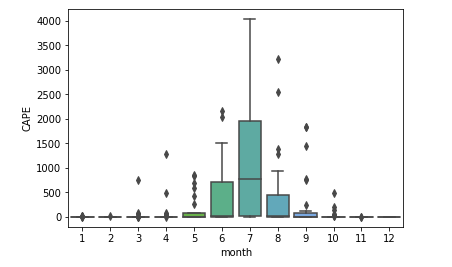
\includegraphics[width=10cm]{00zCAPE.png}
    
\end{center}
\vspace{0.3cm}

\begin{center}
	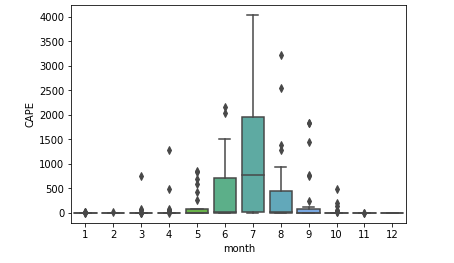
\includegraphics[width=10cm]{12zCAPE.png}
    
\end{center}
\vspace{0.3cm}

\begin{center}
	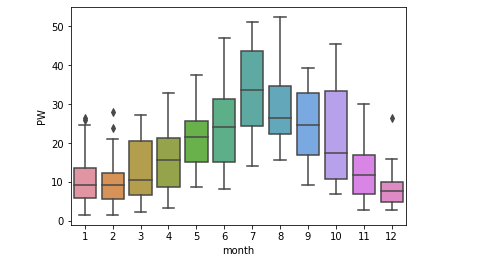
\includegraphics[width=10cm]{00zPW.png}
    
\end{center}
\vspace{0.3cm}

\begin{center}
	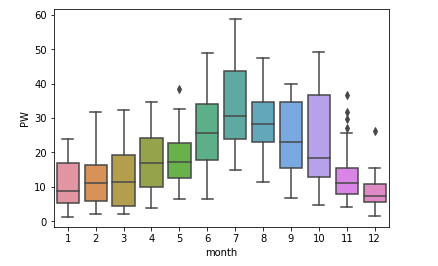
\includegraphics[width=10cm]{12zPW.png}
    
\end{center}
\vspace{0.3cm}

En estas cuatro graficas se usa un Boxplot para cada mes del año. Las primeras dos graficas son de la variable CAPE y las otras dos son de la variable PW. La primera gráfica, de cada variable, es en una hora del día (00z) y la segunda es en otra (12z).

Con estas graficas uno puede obtener la media de los datos, los cuartiles, el rango, si los datos están sesgados a un lado y, si es que hay, datos atípicos del conjunto.  

Como se puede observar, el mes de Julio es en el que se manifiesta una mayor cantidad de PW y un mayor índice de CAPE.

\begin{center}
	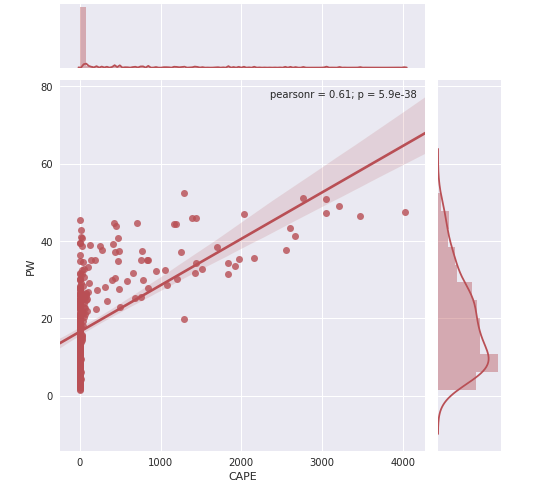
\includegraphics[width=8cm]{00zJointPlot.png}
 
\end{center}
\vspace{0.3cm}

\begin{center}
	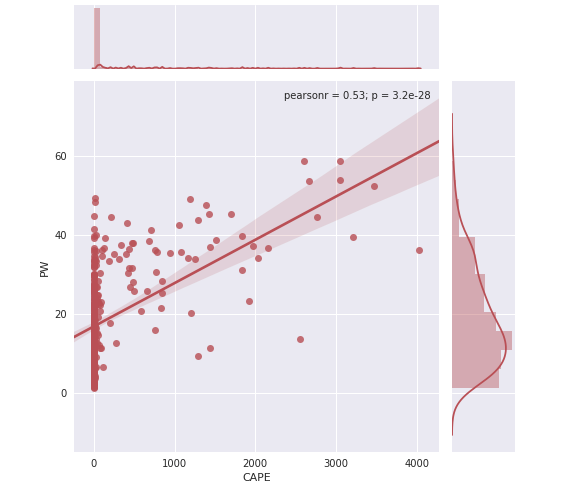
\includegraphics[width=8cm]{12zJointPlot.png}
 
\end{center}
\vspace{0.3cm}

Estas graficas muestran la recta que mejor se ajusta a los puntos en la gráfica, los cuales son de la forma (CAPE\textit{i}, PW\textit{i}).
Junto a las gráficas se encuentran otras dos graficas pequeñas que muestran la distribución de los datos de un eje en la gráfica principal.

En la esquina superior derecha aparece la pendiente de la recta, al igual que en las gráficas pasadas, la primera grafica es de una hora del día (00z) y la otra es de otra hora (12z). 

\begin{center}
	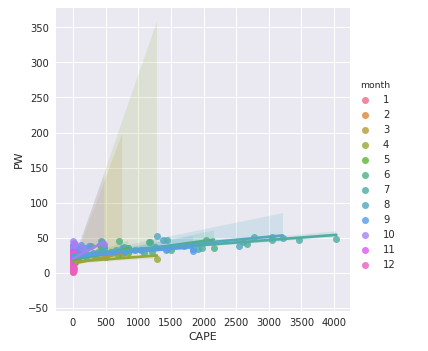
\includegraphics[width=8cm]{00zLmPlot.png}
 
\end{center}
\vspace{0.3cm}

\begin{center}
	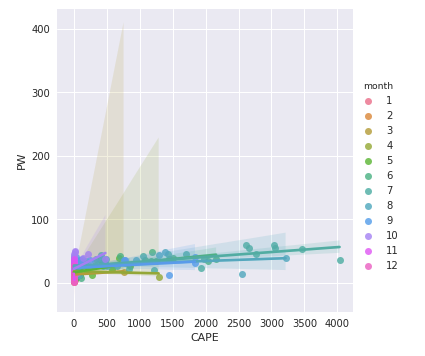
\includegraphics[width=8cm]{12zLmPlot.png}
 
\end{center}
\vspace{0.3cm}

Por último, estos dos graficas muestran doce rectas en cada una, una por cada mes del año, y aparecen unos triángulos que muestran la distribución de los datos, entre más altos estén los triángulos, los datos estarán mas acumulados en ese intervalo.
De la misma manera que en las gráficas pasadas, la primera grafica es de una hora del día (00z) y la otra es de otra hora (12z).  

Como podemos observar, el triángulo del mes de julio es el que llega más lejos, en el que los datos están más distribuidos en la recta. Podemos relacionar esto con lo que vimos en los Boxplots.

\section{Conclusiones}

Después de examinar las gráficas, uno puede llegar a la conclusión que el CAPE y el PW están directamente relacionados, que cuando CAPE aumenta también lo hace PW. Los dos parecen tener su valor máximo en el mes de julio y tienen valores "altos" en los meses cercanos al mes de julio (junio y agosto). EL resto del año, los índices de estas dos variables bajan considerablemente.

\section{Bilbiografía}

\begin{verbatim}
Convective available potential energy. (2018, February 28). 
Retrieved March 01, 2018, from https://en.wikipedia.org/wiki/Convective
_available_potential_energy
\end{verbatim}
%https://en.wikipedia.org/wiki/Convective_available_potential_energy

\begin{verbatim}
Precipitable water. (2018, February 17). Retrieved March 01, 2018, 
from https://en.wikipedia.org/wiki/Precipitable_water 
\end{verbatim}
%https://en.wikipedia.org/wiki/Precipitable_water

\begin{verbatim}
Seaborn: statistical data visualization¶. (n.d.). Retrieved March 03, 2018,
from https://seaborn.pydata.org/index.html
\end{verbatim}
%https://seaborn.pydata.org/index.html

\section{Apéndice}


    1.- ¿Cómo se te hizo esta actividad? ¿Compleja, Difícil, Sencilla?
    
    \vspace{0.3cm}
	Al principio me perdí en las instrucciones de Emacs y no pude seguir el paso, pero al ver cada paso con calma, me di cuenta de que en realidad estaba muy fácil.
    \vspace{0.3cm}
    
\noindent 2.- ¿Qué te llamó más la atención?
    
    \vspace{0.3cm}
	La automatización del proceso de limpieza de un archivo con Emacs y la gran cantidad de graficas que se pueden utilizar en Python para analizar los datos de distintas maneras.
    \vspace{0.3cm}
    
\noindent    3.- ¿Qué parte fue la que menos te interesó hacer?
    
    \vspace{0.3cm}
	El reporte. En verdad me agrado hacer el proceso de limpieza de los datos y las gráficas en Python.
    \vspace{0.3cm}
    
\noindent    4.- ¿Cómo mejorarías esta actividad? ¿Qué le faltó? ¿Qué sobró?
    
    \vspace{0.3cm}
	Al explicar el proceso de limpieza en Emacs, deberíamos de anotar en el pizarrón los comandos más importantes y que la explicación sea un poco más lenta, para que nadie se quede atrás.
    \vspace{0.3cm}
    
\noindent    5.- ¿Hasta este punto, que te parece el uso de Jupyter para programar en Python? 
    
    \vspace{0.3cm}
	Nos proporciona herramientas suficientes para hacer lo que queremos, en este caso, analizar datos de manera gráfica.
    \vspace{0.3cm}


\end{document}